\documentclass[11pt]{article}

\usepackage[utf8]{inputenc}
\usepackage[T1]{fontenc}
\usepackage{lmodern}
\usepackage[margin=1in]{geometry}
\usepackage{setspace}
\usepackage{microtype}
\usepackage{amsmath,amssymb,amsthm,mathtools}
\usepackage{graphicx}
\usepackage{booktabs}
\usepackage{natbib}
\usepackage{placeins}
\usepackage{xurl}
\usepackage[colorlinks=true,linkcolor=blue,citecolor=blue,urlcolor=blue]{hyperref}
\usepackage[nameinlink,capitalize]{cleveref}
\ifdefined\showlinenumbers
  \usepackage[mathlines,switch]{lineno}
\fi

\onehalfspacing
\graphicspath{{figures/}}
\emergencystretch=2em

\newtheorem{theorem}{Theorem}[section]
\newtheorem{proposition}[theorem]{Proposition}
\newtheorem{lemma}[theorem]{Lemma}
\newtheorem{corollary}[theorem]{Corollary}
\theoremstyle{definition}
\newtheorem{assumption}[theorem]{Assumption}
\crefname{assumption}{Assumption}{Assumptions}
\Crefname{assumption}{Assumption}{Assumptions}

\newcommand{\Pbb}{\mathbb{P}}
\newcommand{\Ebb}{\mathbb{E}}
\newcommand{\Fcal}{\mathcal{F}}
\newcommand{\Mcal}{\mathcal{M}}
\newcommand{\Acal}{\mathcal{A}}
\newcommand{\Hcal}{\mathsf{H}}
\newcommand{\Yspace}{\mathsf{Y}}
\newcommand{\norm}[1]{\left\lVert #1\right\rVert}

\title{Extra Hidden States under Emission Misspecification in Hidden Markov Models}
\author{Aur\'elien Nicosia\\
D\'epartement de math\'ematiques et de statistique, Universit\'e Laval\\
Qu\'ebec, Qu\'ebec, Canada\\
\texttt{aurelien.nicosia@mat.ulaval.ca}\\
ORCID: \href{https://orcid.org/0000-0002-0974-9988}{0000-0002-0974-9988}}
\date{}

\begin{document}
\maketitle
\ifdefined\showlinenumbers\linenumbers\fi

\begin{abstract}
Additional hidden Markov states can compensate for restrictive emission
distributions without representing additional scientific regimes. We study
this distinction using the established representation of mixture components
as refined states. Under compactness, mixture identifiability and positive
aggregate transitions, we prove that a simple-emission HMM with too few
components has an observed-law Kullback--Leibler loss that grows at least
linearly with sequence length. An exact refinement, or an aggregate HMM
with mixture emissions, removes this approximation gap. Simulations
illustrate the resulting incentive to add states. An analysis of tumor
allele fractions on chromosome 1 then compares five Gaussian states with
three regional profiles containing five Gaussian components. The fitted
emissions and regional assignments are nearly the same after grouping the
Gaussian states, while the mixture model uses fourteen fewer parameters.
This example illustrates how additional states can describe variation
within a regional profile rather than additional regional regimes. The
number of fitted states alone therefore does not determine the number of
scientifically distinct regimes.

\end{abstract}

\noindent\textit{Keywords:} hidden Markov model; emission misspecification;
finite mixture; relative-entropy rate; state splitting; allelic imbalance.

\medskip
\noindent\textit{MSC 2020:} Primary 62M05; Secondary 62M10.

\section{Introduction}\label{sec:introduction}

Hidden Markov models (HMMs) separate serial dependence from the conditional
distribution of observations through a latent state process. This decomposition
supports applications across time-series analysis, signal processing, and
ecology \citep{Rabiner1989,CappeEtAl2005,ZucchiniEtAl2016}. Fitted states are
often labelled as behaviours, regimes, phases, or classes and then become the
main scientific object reported from an analysis \citep{McClintockEtAl2020}.

That interpretation is useful but not automatic. A fitted state is also part
of a statistical approximation. If the state-dependent distribution is too
restrictive, likelihood can improve by creating states whose emissions jointly
approximate skewness, heavy tails, overdispersion, or within-regime
heterogeneity. An additional state can therefore be statistically useful
without representing an additional scientific regime. Under misspecification,
likelihood targets a best approximation in the fitted family rather than the
data-generating parameter \citep{White1982,DoucMoulines2012}.

The practical phenomenon is established in the HMM literature.
\citet{PohleEtAl2017} show that information criteria can favour state counts
that are difficult to interpret scientifically. Additional states may absorb
unmodelled structure in state-dependent distributions, while flexible
parametric, mixture, and nonparametric observation models offer alternatives
\citep{Dannemann2012,DannemannEtAl2014,LangrockEtAl2015,LangrockEtAl2018}.
The distinction matters because methods for estimating statistical HMM order
\citep{GassiatKeribin2000,GassiatRousseau2014,Lehericy2019,ZouEtAl2024,LinHuang2025}
do not imply that every selected state is a distinct scientific regime.

Mixture-emission estimation and component aggregation already have a substantial
methodological basis. \citet{VolantEtAl2014} give the component-state
representation and an EM-based merging approach. \citet{HolzmannSchwaiger2015}
characterize minimal representations and test whether states can be reduced
to mixture components without changing the observed law. We use this
established refinement construction as the starting point, not as a new
model or estimation algorithm.

Our result concerns uniform separation from a restrictive emission class.
Under compactness, identifiable mixture order and positive aggregate
transitions, every one-step true predictive density remains a positive
$L^1$ distance from every mixture with only the aggregate number of simple
components. The chain rule turns this bound into a Kullback--Leibler divergence that is
at least proportional to sequence length against every HMM in the smaller
class, without aligning hidden paths or restricting candidate transitions.
Marginal mixture identifiability already establishes non-representability.
The additional predictive bound gives uniform separation at every sequence
length and a positive relative-entropy-rate gap. The result
complements HMM likelihood and identifiability theory
\citep{Leroux1992,BickelEtAl1998,AllmanEtAl2009,GassiatEtAl2016,AlexandrovichEtAl2016}.

The empirical comparison asks whether an additional state is needed to
describe a new regime or to represent variation within an existing one.
We compare ordinary and mixture-emission HMMs, including pairs with the
same total number of Gaussian components. Holding this count fixed isolates
the additional freedom in the transition model. A simulation shows the
mechanism when the aggregate states are known. The application examines
chromosome-1 tumor allele fractions: low and high fractions at successive
markers can describe the same regional imbalance. This gives a scientific
reason to group two emission components within one Markov state. The
Supporting Information contains further genomic comparisons and an elk
movement example that examines sensitivity to the emission family.

Section~\ref{sec:mechanism} gives the formal mechanism; Sections~\ref{sec:em}
and~\ref{sec:workflow} describe estimation and model comparison; and
Sections~\ref{sec:simulation} and~\ref{sec:genomic} illustrate the comparison in
simulation and data.

\section{Why restrictive emissions create extra states}\label{sec:mechanism}

If a scientifically meaningful regime has a heterogeneous emission distribution, several simple-emission
states can improve fit by representing its components rather than by revealing
new regimes. The formal results below give conditions under which an
aggregate-state model with richer emissions and a refined model with additional
simple-emission states generate the same observed process.

Let $\Yspace$ be the observation set, let $\mathcal B$ be its sigma-field, let
$\lambda$ be a dominating measure on $(\Yspace,\mathcal B)$, and let $\Theta$
be the emission-parameter space. All
densities below are with respect to $\lambda$. For densities $p$ and $q$, define
the Kullback--Leibler divergence and the $L^1(\lambda)$ distance by
\begin{equation*}
 D(p\Vert q)=\int_{\Yspace}p(y)\log\!\left\{\frac{p(y)}{q(y)}\right\}\lambda(dy),
 \qquad
 \norm{p-q}_1=\int_{\Yspace}|p(y)-q(y)|\lambda(dy).
\end{equation*}
Here, $0\log(0/q)=0$, and $D(p\Vert q)=+\infty$ if $q=0$ on a set having
positive probability under $p$. The same notation $D(P\Vert Q)$ is used for
probability laws through their densities. Let
$\Fcal=\{f_\eta:\eta\in\Theta\}$ be the simple fitted emission family. Define
the class of mixtures with at most $K$ atoms, for an integer $K\geq1$, by
\begin{equation*}
 \Mcal_K=\left\{\sum_{j=1}^K\omega_j f_{\eta_j}:
 \omega_j\geq0,\ \sum_{j=1}^K\omega_j=1,\ \eta_j\in\Theta\right\}.
\end{equation*}
Thus, the $\omega_j$ are mixing proportions. Zero weights are permitted, so
$\Mcal_K\subseteq\Mcal_{K+1}$. Let $\Hcal_K(\Fcal)$ denote the observed
process laws generated by $K$-state HMMs with emissions in $\Fcal$, arbitrary
transition matrices, and arbitrary initial distributions. For process laws $P$
and $Q$, let $P^{1:T}$ and $Q^{1:T}$ denote the respective joint laws of
$(Y_1,\ldots,Y_T)$ and write
\begin{equation*}
 \underline D^{\mathrm{rate}}(P\Vert Q)
 =\liminf_{T\to\infty}T^{-1}D(P^{1:T}\Vert Q^{1:T})
\end{equation*}
for their lower relative-entropy rate.

Fix an integer $K_0\geq1$, interpreted as the number of aggregate scientific
regimes. A superscript $0$ denotes a data-generating parameter. The
following assumptions isolate a transparent finite-mixture setting.

\begin{assumption}[Emission regularity]\label{ass:regularity}
The parameter space $\Theta$ is compact, the map $\eta\mapsto f_\eta$ is
continuous into $L^1(\lambda)$, and every $f_\eta$ is positive
$\lambda$-almost everywhere.
\end{assumption}

\begin{assumption}[Identifiable mixture order]\label{ass:identifiability}
Finite mixtures from $\Fcal$ have identifiable minimal order. Two equal finite
mixtures with positive weights and pairwise distinct parameters have the same
number of components and agree up to permutation.
\end{assumption}

Classical sufficient conditions are given by \citet{Teicher1963} and
\citet{YakowitzSpragins1968}; see also \citet{McLachlanPeel2000}. The
assumptions include univariate Gaussian emissions on compact mean and variance
sets with variances bounded away from zero.

\begin{lemma}[Separation from lower-order mixtures]\label{lem:separation}
Under Assumptions~\ref{ass:regularity} and~\ref{ass:identifiability}, let
$R>K_0$ be an integer and let $\eta_1^0,\ldots,\eta_R^0\in\Theta$ be pairwise distinct.
For $c>0$ and
$Rc\leq1$, set
\begin{equation*}
 \Acal_c=\left\{\sum_{r=1}^R\omega_r f_{\eta_r^0}:
 \omega_r\geq c,\ \sum_{r=1}^R\omega_r=1\right\}.
\end{equation*}
Then $d_c:=\inf_{p\in\Acal_c}\inf_{q\in\Mcal_{K_0}}\norm{p-q}_1>0$, and
\begin{equation*}
 \inf_{p\in\Acal_c}\inf_{q\in\Mcal_{K_0}}D(p\Vert q)
 \geq d_c^2/2>0.
\end{equation*}
\end{lemma}

The lemma says that a mixture containing $R$ distinct atoms, each with a
non-negligible weight, cannot be approximated arbitrarily closely by only
$K_0<R$ atoms.

To see the approximation incentive directly, let $Z_t\in\{1,\ldots,K_0\}$ be
a stationary aggregate Markov chain with transition matrix
$\Gamma^0=(\gamma^0_{k\ell})$ and stationary probabilities
$\pi_k=\Pbb(Z_t=k)>0$. Here,
$\gamma^0_{k\ell}=\Pbb(Z_t=\ell\mid Z_{t-1}=k)$. Suppose the emission in state
$k$ is $g_k$, and, for an integer $m\geq1$, define
$\delta_k(m)=\inf_{q\in\Mcal_m}D(g_k\Vert q)$. Thus,
$\delta_k(m)$ is the infimum of the emission-level Kullback--Leibler loss
with at most $m$ atoms from $\Fcal$. For specified aggregate-state
emissions $q_1,\ldots,q_{K_0}$, define the aligned risk by
\begin{equation*}
 \mathcal{R}(q_1,\ldots,q_{K_0})=\sum_{k=1}^{K_0}\pi_k D(g_k\Vert q_k).
\end{equation*}
This comparison fixes the law of the aggregate hidden trajectory. In the
refined representation, the within-state component is drawn independently
at each visit, conditional on the aggregate states; the emission $q_k$ can
therefore be any member of $\Mcal_{m_k}$.

\begin{proposition}[Aligned improvement by state splitting]\label{prop:aligned}
If aggregate state $k$ is represented by one emission from $\Fcal$, the infimum of the
aligned Kullback--Leibler risk is
$\sum_{k=1}^{K_0}\pi_k\delta_k(1)$. If it is represented by $m_k\geq1$
substates, where $m_k$ is the number allocated to aggregate state $k$, the infimum of the
aligned risk is $\sum_{k=1}^{K_0}\pi_k\delta_k(m_k)$. If $\sum_k\pi_k\delta_k(1)<\infty$, the second risk is
strictly smaller whenever
$\delta_{k^\star}(m_{k^\star})<\delta_{k^\star}(1)$ for at least one state.
\end{proposition}

State splitting gives a heterogeneous state several emission atoms
instead of one. The statement is only an aligned comparison because it holds
the aggregate trajectory law fixed; attainment of the infima is not required. The next construction removes that
restriction.

We recall the component-state construction of \citet{VolantEtAl2014};
see also \citet{HolzmannSchwaiger2015}. Suppose each aggregate emission is a
finite mixture with $m_k$ components and $\eta^0_{k,a}\in\Theta$,
\begin{equation}\label{eq:true-emissions}
 g_k(y)=\sum_{a=1}^{m_k}\omega^0_{k,a}f_{\eta^0_{k,a}}(y),
 \qquad \omega^0_{k,a}>0,\quad \sum_a\omega^0_{k,a}=1.
\end{equation}
The $\omega^0_{k,a}$ are the within-state mixing proportions.

\begin{proposition}[Exact HMM refinement]\label{prop:refinement}
Let the refined states be $(k,a)$, where $1\leq k\leq K_0$ and
$1\leq a\leq m_k$. Give state $(k,a)$ emission
$f_{\eta^0_{k,a}}$ and transition probabilities
\begin{equation}\label{eq:refined-transition}
 \Gamma^{\mathrm{ref}}_{(k,a),(\ell,b)}
 =\gamma^0_{k\ell}\omega^0_{\ell,b}.
\end{equation}
With initial probabilities $\pi_k\omega^0_{k,a}$, the refined HMM has exactly
the same observed process law as the aggregate HMM with transitions
$\Gamma^0$ and emissions in~\eqref{eq:true-emissions}.
\end{proposition}

Equation~\eqref{eq:refined-transition} retains the probability of moving from
aggregate state $k$ to $\ell$, then draws a component of the destination
emission. The refined states therefore encode within-regime mixture components,
not new aggregate dynamics.

For the genomic example in Section~\ref{sec:genomic}, the component counts
$(2,2,1)$ give three aggregate states and five refined states. The two
components of each paired state have different emissions but share the same
transition row in the refined representation. An unrestricted five-state
HMM can instead give each component its own transition row. This is the
specific restriction examined in the application.

Assume now that
$\varepsilon:=\min_{1\leq k,\ell\leq K_0}\gamma^0_{k\ell}>0$, let
$R=\sum_{k=1}^{K_0}m_k$, let
$\omega_{\min}=\min_{1\leq k\leq K_0,\,1\leq a\leq m_k}\omega^0_{k,a}$, and set
$c=\varepsilon\omega_{\min}$. Suppose $R>K_0$ and all
$\eta^0_{k,a}\in\Theta$ are pairwise distinct.

\begin{theorem}[Observed-law separation]\label{thm:separation}
Under Assumptions~\ref{ass:regularity} and~\ref{ass:identifiability}, the
stationary aggregate HMM with emissions~\eqref{eq:true-emissions} has observed
law $P_0^Y$. For every integer $T\geq1$ and every
$Q\in\Hcal_{K_0}(\Fcal)$,
\begin{equation}\label{eq:finite-separation}
 D\{(P_0^Y)^{1:T}\Vert Q^{1:T}\}\geq T d_c^2/2.
\end{equation}
Consequently,
\begin{equation*}
 \inf_{Q\in\Hcal_R(\Fcal)}
 \underline D^{\mathrm{rate}}(P_0^Y\Vert Q)=0,
 \qquad
 \inf_{Q\in\Hcal_{K_0}(\Fcal)}
 \underline D^{\mathrm{rate}}(P_0^Y\Vert Q)\geq d_c^2/2>0.
\end{equation*}
\end{theorem}

The constant is uniform over the candidate HMMs, but depends on the fixed
true atoms, their minimum weight, the transition bound and the compact
fitted parameter set. It need not stay bounded away from zero when distinct
atoms approach one another or these lower bounds vanish.

The first equality follows because the refined $R$-state model reproduces the
truth exactly. For the second, every one-step prediction from a $K_0$-state
simple-emission HMM belongs to $\Mcal_{K_0}$, while every true prediction
contains all $R$ atoms with weights at least $c$. The mixture separation lemma
and the chain rule for relative entropy give~\eqref{eq:finite-separation}
for every $T$, hence the positive rate gap. This
argument concerns observed predictive distributions and does not align hidden
paths.

More generally, for any integer $1\leq K<R$, define
$d_{c,K}:=\inf_{p\in\Acal_c}\inf_{q\in\Mcal_K}\norm{p-q}_1>0$.
The same argument gives
$D\{(P_0^Y)^{1:T}\Vert Q^{1:T}\}\geq T d_{c,K}^2/2$
for every $Q\in\Hcal_K(\Fcal)$. The constant depends on $K$;
$d_{c,K_0}=d_c$. Thus the approximation gap persists whenever the candidate
has fewer states than the true number of distinct emission components,
not only when it has $K_0$ states. Supporting Information S1.4 gives the
argument for this extension.

\begin{corollary}[Enriched-emission representation]\label{cor:enriched}
If the fitted emission family is enlarged from $\Fcal$ to $\Mcal_M$, with an
integer $M\geq\max_{1\leq k\leq K_0}m_k$, then
\begin{equation*}
 \inf_{Q\in\Hcal_{K_0}(\Mcal_M)}
 \underline D^{\mathrm{rate}}(P_0^Y\Vert Q)=0.
\end{equation*}
\end{corollary}

Thus, a refined model with more simple-emission states and an aggregate model
with richer emissions can describe the same observations. Equality of the two
representations does not determine which latent description is scientifically
meaningful.

A likelihood-selection consequence requires an additional stochastic limit,
not just a bound on expected divergence. For example, suppose the normalized
log-likelihood ratios $T^{-1}\log\{p_0(Y_{1:T})/q(Y_{1:T})\}$ converge almost
surely, uniformly over $Q\in\Hcal_{K_0}(\Fcal)$, to limits bounded below by
$d_c^2/2$. Then the maximized log-likelihood advantage of the $R$-state class
is at least $T(d_c^2/2-o(1))$, since this class contains the truth. Any fixed
parameter-count BIC penalty difference is only of order $\log T$.
Under that additional assumption, BIC eventually prefers $R$ to $K_0$
simple-emission states. This conditional comparison neither proves the
uniform convergence assumption nor selects $R$ against every other order.

For reference, Sections~S1.1--S1.5 of the Supporting Information give proofs
of Lemma~2.3, Proposition~2.4, Proposition~2.5, Theorem~2.6, and
Corollary~2.7, respectively.

\section{Fitting the enriched-emission HMM}\label{sec:em}

Let $X_t\in\{1,\ldots,K\}$ denote the fitted hidden state at time $t$. For
state $k$, let $M_k\geq1$ be the number of fitted Gaussian components and let
$\phi(y;\mu,\sigma^2)$ denote the Gaussian density at $y$ with mean $\mu$ and
variance $\sigma^2>0$. The fitted state-dependent density is
\begin{equation*}
 b_k(y)=\sum_{m=1}^{M_k}\omega_{km}
 \phi(y;\mu_{km},\sigma_{km}^2),
 \qquad \omega_{km}\geq0,\quad \sum_m\omega_{km}=1.
\end{equation*}
The quantities $\omega_{km}$ are mixing proportions within state $k$; they do
not change the state transition probabilities. The hidden chain has initial
probabilities $\alpha_k=\Pbb(X_1=k)$ and transition probabilities
$a_{k\ell}=\Pbb(X_t=\ell\mid X_{t-1}=k)$, collected in
$A=(a_{k\ell})$.

The following standard mixture-emission expectation-maximization (EM)
updates are included to specify the fitted model \citep{VolantEtAl2014}.
The algorithm alternates between state and component allocation and
closed-form parameter updates. Write
$Y_{1:T}=(Y_1,\ldots,Y_T)$ and let $C_t\in\{1,\ldots,M_{X_t}\}$ denote the
Gaussian-component label at time $t$. A scaled forward--backward recursion gives
\begin{align*}
 \zeta_t(k)&=\Pbb(X_t=k\mid Y_{1:T}),\\
 \xi_t(k,\ell)&=\Pbb(X_{t-1}=k,X_t=\ell\mid Y_{1:T}).
\end{align*}
Here, $\zeta_t(k)$ is defined for $t=1,\ldots,T$, whereas
$\xi_t(k,\ell)$ is defined for $t=2,\ldots,T$.
The joint posterior responsibility for state $k$ and component $m$ is
\begin{equation*}
 r_t(k,m)=\Pbb(X_t=k,C_t=m\mid Y_{1:T})=\zeta_t(k)
 \frac{\omega_{km}\phi(Y_t;\mu_{km},\sigma_{km}^2)}{b_k(Y_t)}.
\end{equation*}
The M-step updates are
\begin{align*}
 \alpha_k^{\mathrm{new}}&=\zeta_1(k), &
 a_{k\ell}^{\mathrm{new}}&=
 \frac{\sum_{t=2}^T\xi_t(k,\ell)}
 {\sum_{t=2}^T\sum_j\xi_t(k,j)},\\
 \omega_{km}^{\mathrm{new}}&=
 \frac{\sum_t r_t(k,m)}{\sum_t\zeta_t(k)}, &
 \mu_{km}^{\mathrm{new}}&=
 \frac{\sum_t r_t(k,m)Y_t}{\sum_t r_t(k,m)},\\
 (\sigma_{km}^2)^{\mathrm{new}}&=
 \frac{\sum_t r_t(k,m)(Y_t-\mu_{km}^{\mathrm{new}})^2}
 {\sum_t r_t(k,m)}.
\end{align*}
In these updates, sums over $t$ without displayed limits run from $1$ to $T$,
and $\sum_j$ runs over the $K$ fitted states.
For independent sequences with common parameters, the forward--backward
recursion resets at each sequence start. The initial-probability update is
the average of the state responsibilities at those starts; transition sums
exclude boundaries, while emission sums pool all observations. Numerical
pseudocounts and variance constraints are specified in SI S2--S3.
In computation, a small lower bound on $\sigma_{km}$ prevents likelihood
degeneracy. Multiple starts are needed because mixture-HMM likelihoods are
multimodal. For a sequence of length $T$, BIC is
$-2\ell(\widehat\theta)+p\log T$, where $\widehat\theta$ is the maximum
likelihood estimate, $\ell(\widehat\theta)$ is the maximized log-likelihood,
and the number $p$ of free parameters is
\begin{equation*}
 (K-1)+K(K-1)+\sum_{k=1}^K\{(M_k-1)+2M_k\}.
\end{equation*}
The three terms count initial probabilities, transition probabilities, and
state-specific mixture parameters, respectively.

\section{Comparing emission and transition complexity}\label{sec:workflow}

Suppose scientific knowledge suggests $K_0$ aggregate regimes, while a
simple-emission analysis favours additional states. A $K_0$-state HMM with
$R=\sum_k M_k$ Gaussian components is an $R$-state Gaussian HMM whose
transition probabilities satisfy the refinement constraints in
Proposition~\ref{prop:refinement}, with initial probabilities
$\alpha^{\mathrm{ref}}_{(k,m)}=\alpha_k\omega_{km}$. Comparing it with an unrestricted
$R$-state model holds the emission component count fixed and changes the
latent dynamics. For example, two aggregate states with component counts
$(2,1)$ have 10 free parameters, compared with 14 for three Gaussian states;
counts $(2,2)$ give 13, compared with 23 for four Gaussian states. A comparison
of two states with four components against three Gaussian states changes both
the component count and the transition structure.

The factorization requires both equal transition rows within each source
group and destination-component proportions that do not depend on the source
state. Equal rows or a low matrix rank alone do not establish the full
constraint \citep{HolzmannSchwaiger2015}. We specify the groups from the
emission mechanism, then compare the constrained and unrestricted fits.
The state-reduction test of \citet{HolzmannSchwaiger2015} addresses this
question under a stationary initial law. For the genomic comparison we
use a model-conditional parametric bootstrap with the fitted initial law;
Supporting Information S3.2 explains its calibration and limitations.

BIC summarizes penalized likelihood within the specified model classes.
It is not a test of the number of biological regimes. In particular, mixture
singularities and transition estimates near the boundary limit a regular
asymptotic interpretation of its penalty. An unrestricted refined fit must
have likelihood at least as high as the corresponding constrained fit at a
common variance bound; initialization at the exact refinement provides a
numerical check of that nesting.

Prediction is assessed separately from fit. Parameters estimated on the
training data are held fixed while the filter incorporates observations in
an evaluation sequence. Its sequential log score is
$\sum_t\log p_{\widehat\theta}(Y_t\mid Y_{1:t-1})$, with the fitted initial
law used at a new sequence start. Higher scores indicate better predictive
densities on that sequence. For a continuation of a training sequence, the
filter instead continues from the training endpoint. Probability integral
transforms and interval coverage provide further descriptive checks in the
Supporting Information. Similar log scores alone do not establish predictive
equivalence.

Decoded sequences and state-dependent distributions connect these comparisons
to the observations. Cross-tabulations indicate when two Gaussian states map
largely to one mixture-emission state, but do not establish that the latter is
scientifically correct. States index Markov dynamics; mixture components
describe within-state distributions; modes are local maxima of a density.
These three counts need not coincide. Interpretation therefore also depends
on temporal stability, sensitivity to fitting constraints, and measurements
relevant to the scientific question.

\section{Simulation study}\label{sec:simulation}

We write G$K$ for a $K$-state Gaussian HMM. For mixture-emission models,
the digits after M give the component counts in successive states: M21
has counts $(2,1)$, M22 has $(2,2)$, and M221 has $(2,2,1)$.

We first isolate the mechanism in a controlled setting. The data-generating
process has two aggregate states, transition matrix
\begin{equation*}
 \Gamma^0=\begin{pmatrix}0.93&0.07\\0.05&0.95\end{pmatrix}.
\end{equation*}
The first-state emission was a two-component Gaussian mixture with weights
0.70 and 0.30, means $-1.20$ and $1.10$, and standard deviations 0.55 and
0.45. The second-state emission was Gaussian with mean 3.80 and standard
deviation 0.65. The process therefore
has two aggregate regimes and three distinct Gaussian atoms.

For a reference series of length 1500, we fitted Gaussian HMMs with $K=2$ and
$K=3$, and an enriched $K=2$ HMM with two Gaussian components per state. Each
model was fitted with the protocol used for the replications below. The two-state Gaussian model merged the heterogeneous
first regime and had BIC 4487.4. The three-state Gaussian model separated its
two components and had BIC 4197.3. The enriched two-state model recovered the
same within-regime structure while retaining two aggregate states and had BIC
4191.6. \Cref{fig:simulation-density} shows the directly observable emission
fit.

\begin{figure}[tbp]
\centering
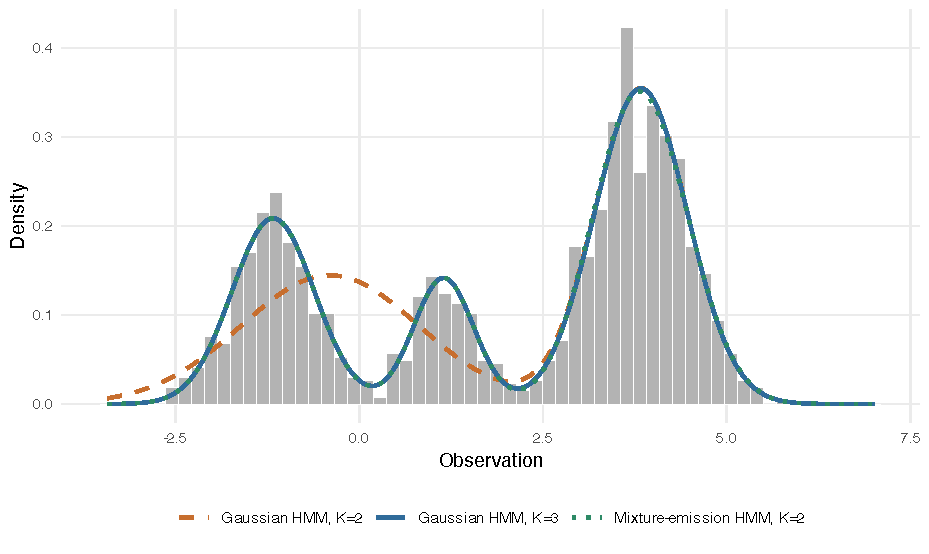
\includegraphics[width=.78\linewidth]{simulation_density.pdf}
\caption{Observed histogram and fitted marginal densities for the reference
simulation. The two-state Gaussian model smooths over the heterogeneous first
regime. The three-state Gaussian and enriched two-state models recover its two
components.}
\label{fig:simulation-density}
\end{figure}

Across 200 fixed-seed replications at each sample size, BIC preferred the
three-state to the two-state Gaussian model in 99.5\%, 100\% and 100\% of
samples for $T=500,1500,5000$, respectively. Comparing G3 with the enriched
two-state model, BIC preferred the latter in 96.0\%, 99.0\% and 99.5\%.
Both classes contain the data-generating law. Their fitted log likelihoods
are nearly equal on average, and the mean M22-minus-G3 BIC differences
$-6.5,-7.7,-8.6$ are close to $-\log T$. The preference mainly reflects
M22's smaller parameter count (13 versus 14), rather than a substantial
improvement in fit.
An initial fitting protocol preferred G2 over G3 by BIC in 40 of the 600
replications. The reported fits use additional data-derived starts and
refinement to relative likelihood tolerance $10^{-9}$. In particular, an
exact refinement of a fitted M21 model supplies a G3 start without using
generating parameters. This improved optimization changes 39 of those 40
preferences to G3: the initial G2 preferences mainly reflected incomplete
optimization. SI S2 documents both protocols and the retained fits.
The enriched candidate has four components although the
data-generating distribution has three; these frequencies therefore do not
isolate the equal-component comparison of Section~\ref{sec:workflow}.
That comparison is implemented directly in the genomic analysis. Full
computational details and additional diagnostics are reported in the Supporting Information.

These frequencies are descriptive. Finite mixtures and overfitted HMMs contain
singular parameter strata, so regular-model interpretations of BIC require
caution \citep{Keribin2000,RousseauMengersen2011,GassiatRousseau2014,Watanabe2013,DrtonPlummer2017}.

\section{Chromosomal allelic imbalance}\label{sec:genomic}

\subsection{Question and models}\label{sec:genomic-question}

We analyze chromosome 1 of the breast-cancer cell line HCC1143 and its
matched normal cell line HCC1143BL, using the SNP-array measurements of
\citet{ChiangEtAl2009}. At a single-nucleotide polymorphism (SNP), the
B-allele fraction is the B signal divided by the combined A and B signals.
The measurements are unphased: the allele labelled B need not come from the
same parental chromosome at successive markers. Consequently, fractions
near 0.2 and 0.8 can describe the same regional allelic imbalance
\citep{OlshenEtAl2011}. A mixture emission can represent these two bands
within one regional profile. The question is whether the bands require
separate transition dynamics. Data details are given in Supporting
Information S3.1.

We fit G2--G5, M21 and M221 to 20,697 ordered markers. Each Markov state
of a mixture model represents a regional profile, corresponding to an
aggregate regime in Section~\ref{sec:mechanism}.
The M21/G3 and M221/G5 comparisons hold the total
number of Gaussian components fixed. In particular, M221 corresponds to
$K_0=3$ and $R=5$ in Proposition~\ref{prop:refinement}. G5 relaxes its
component-group transition and initial-distribution constraints, adding
14 parameters without adding emission components. If an M221 process
satisfied the assumptions of Theorem~\ref{thm:separation}, its extension
to $K<R$ would give a positive approximation gap for G2--G4. This motivates
examining emission complexity; the fitted data do not verify those assumptions.
Multiple starts and
numerical checks are documented in Supporting Information S3.2.

\subsection{Chromosome-1 results}\label{sec:genomic-results}

\begin{table}[htbp]
\centering
\small
\caption{Chromosome-1 comparison. $K$ is the number of Markov states, $R$ the total number of Gaussian components, and $p$ the number of free parameters. Lower BIC is preferred. Repeat scores are sequential log scores on chromosome 1 of the second array pair, with fitted parameters held fixed; higher scores are preferred. This is a technical repeat of the same cell lines.}
\label{tab:genomic-comparison}
\begin{tabular}{lrrrrr}
\toprule
Model & $K$ & $R$ & $p$ & BIC & Repeat score \\
\midrule
G2 & 2 & 2 & 7 & -14751.5 & 7049.59 \\
G3 & 3 & 3 & 14 & -20738.2 & 9818.62 \\
G4 & 4 & 4 & 23 & -22415.1 & 10767.74 \\
G5 & 5 & 5 & 34 & -24697.0 & 11907.57 \\
M21 & 2 & 3 & 10 & -20773.1 & 9816.15 \\
M221 & 3 & 5 & 20 & -24817.8 & 11906.57 \\
\bottomrule
\end{tabular}
\end{table}


M221 estimates paired component centres at $(0.185,0.805)$ and
$(0.392,0.601)$, and a single centre at 0.498. We call these strong imbalance,
moderate imbalance and approximate balance, respectively. These names
describe the measured fractions, not cell populations or absolute DNA copy
numbers. Figure~\ref{fig:genomic-profiles} shows both the regional profiles
and the Gaussian components within them.

G4 improves on G3, but its BIC remains 2402.7 higher than M221's.
Among G2--G5, G5 has the lowest BIC. The more informative comparison for
the refinement construction is G5 versus M221: G5 estimates almost the
same five component distributions, gains only 9.13 log-likelihood units,
and has a BIC 120.87 higher. Thus, on this chromosome the additional
component-level transition freedom produces little improvement in fit.
A model-conditional parametric bootstrap under M221 gives a likelihood-ratio
statistic of 18.26 and a Monte Carlo p-value of 0.09 from 199 replicates
(Supporting Information S3.2), without rejecting the refinement constraints
at the 5\% level.

The raw G5 Viterbi path has 9,123 runs, compared with 181 for M221.
Many G5 switches are between the low and high bands within the same regional
profile. Matching the Gaussian emissions and grouping the paired G5 states
gives 99.73\% agreement with M221 and 194 runs. The ordinary HMM therefore
recovers nearly the same regional description after aggregation; the
mixture model represents that grouping directly in its Markov structure.

\begin{figure}[htbp]
\centering
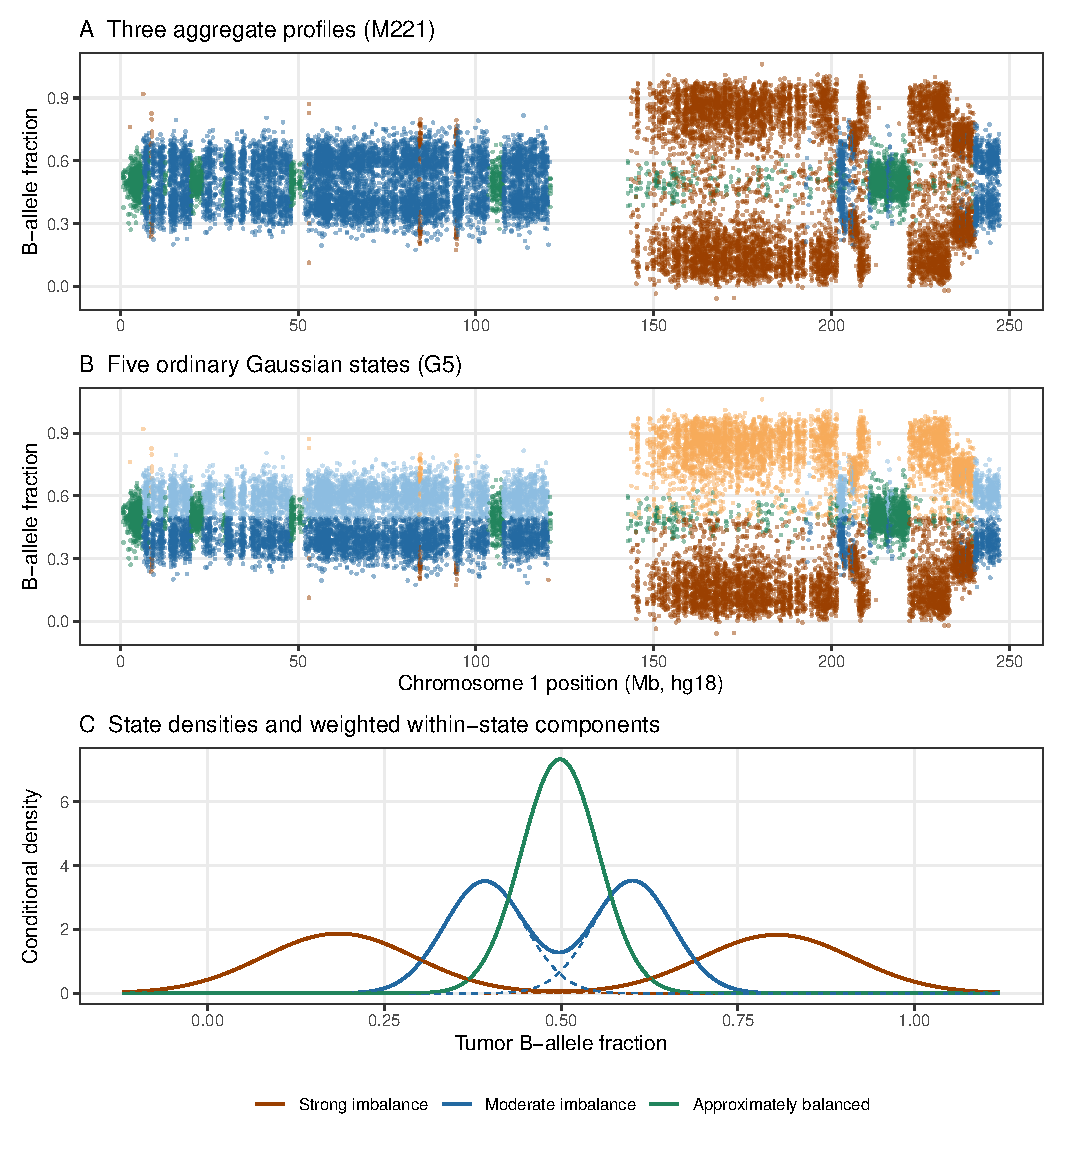
\includegraphics[width=.94\linewidth]{genomic_profiles.pdf}
\caption{Chromosome 1 of HCC1143. Panels A and B colour allele fractions by
the M221 and G5 Viterbi paths. Paired light and dark colours in B distinguish
Gaussian states belonging to the same aggregate colour in A. Panel C shows
M221 state densities (solid) and weighted component contributions (dashed).
The densities are conditional on the aggregate state.}
\label{fig:genomic-profiles}
\end{figure}

A second array pair measures the same cell lines again. With the
chromosome-1 estimates held fixed, M221 and G5 have almost identical
sequential log scores on this technical repeat (Table~\ref{tab:genomic-comparison}).
The M221 paths decoded from the first and second array pairs assign the
same regional profile to 98.08\% of the 19,727 shared markers.
These results assess repeatability within this cell line, not performance
across patients or accuracy against known regional states.

The application illustrates the distinction between emission components and
regional dynamics. It does not establish that three is the true number of
regional regimes. Unequal marker spacing and residual dependence also limit
the interpretation of individual short runs. Supplementary analyses include
prediction and calibration (S3.3), repeatability and sensitivity (S3.4),
models incorporating allelic symmetry (S3.5), and comparisons with genomic
segmentation and independent sequencing (S3.6). S3.3 identifies evaluation
sequences on which other models predict better; S3.5 reports the fit and
prediction trade-offs of imposing symmetry. S3.6 examines how the inferred
profiles relate to measurements from other methods.

\FloatBarrier

\section{Discussion}\label{sec:discussion}

The theoretical result separates the number of emission components from the
number of aggregate regimes. When the aggregate emissions contain more
identifiable components than an ordinary HMM can supply, the assumptions
of Theorem~\ref{thm:separation} imply a positive predictive approximation
gap. Extra simple-emission states can remove this gap through the exact
refinement construction. They need not introduce new aggregate dynamics.

The simulation illustrates this mechanism with known aggregate states. The
genomic application examines its practical counterpart: whether low and
high allele-fraction bands need separate regional transition laws. M221
and G5 fit nearly the same component distributions and yield nearly the
same regional assignments after aggregation. M221 makes the grouping
explicit and uses fewer parameters. The data illustrate the construction;
they do not verify all assumptions of the separation theorem or identify a
unique biological state count.

Comparisons should therefore distinguish improved emission fit from evidence
for additional regimes. At a fixed component count, the constrained and
unrestricted models isolate additional freedom in the latent dynamics.
BIC, predictive scores and decoded paths then answer different questions.
On chromosome 1, M221 has the lower BIC while G5 has a slightly higher
technical-repeat score (Table~\ref{tab:genomic-comparison}); neither criterion
alone establishes the regional interpretation.
In particular, nonrejection of the refinement constraints in the
model-conditional bootstrap is not an equivalence result.

The formal result assumes finite mixtures, a compact fitted emission family
and positive aggregate transitions. Its separation constant can shrink as
components approach one another or lower weight and transition bounds vanish.
Heavy-tailed or skewed emissions may require increasingly rich approximations
rather than a finite exact refinement. Structural zeros would require an
accessibility argument in place of the uniform one-step bound. The theorem
also does not establish finite-sample state recovery or BIC consistency;
the likelihood-selection implication stated in Section~\ref{sec:mechanism}
requires an additional uniform stochastic limit.

More generally, extra states can absorb omitted covariates, misspecified
transitions or unresolved temporal structure as well as restrictive
emissions. The supplementary elk analyses illustrate sensitivity to these
modeling choices. Scientific interpretation therefore requires domain
knowledge and measurements beyond fitted state labels
\citep{PohleEtAl2017,McClintockEtAl2020}. Neither equivalent observed laws
nor similar fitted partitions determine a unique scientific interpretation
of the hidden process.

\section{Conclusion}\label{sec:conclusion}

A simple-emission HMM can gain useful states because its emission family is
too restrictive. Exact refinement and the predictive separation bound
explain how this can occur without additional aggregate regimes. Comparing
ordinary and mixture-emission models at a fixed component count makes the
extra freedom in latent dynamics explicit. In the chromosome-1 example,
M221 represents three regional profiles using five Gaussian components.
Grouping the five G5 states gives nearly the same regional assignments.
The scientific meaning of
those profiles must be assessed separately from the number of fitted states.

\section*{Acknowledgments}\label{sec:acknowledgments}
OpenAI ChatGPT and Codex were used for manuscript drafting and revision,
including the genomic application, and for assistance with code development
and numerical checks. The author is responsible for the mathematical
arguments, verification and interpretation of results, and the final
manuscript.

\section*{Funding}
This research did not receive any specific grant from funding agencies in the
public, commercial, or not-for-profit sectors.

\section*{Data availability statement}
The SNP-array data are publicly available in Gene Expression Omnibus,
accession GSE13372, at
\url{https://www.ncbi.nlm.nih.gov/geo/query/acc.cgi?acc=GSE13372}.
Sequencing segment estimates are in the supplementary materials of
\citet{ChiangEtAl2009}. The accompanying reproducibility package contains
processed marker tables, fitted models, scripts, fixed seeds, source hashes
and numerical tests for the simulations, genomic application and
supplementary elk analyses. It documents regeneration from the original CEL files
and annotation files, as well as reproduction from the supplied processed
inputs. The project repository is
\url{https://github.com/AurelienNicosiaULaval/corrective-hmm-states}.
The package documents the original sources for each data set.

\section*{Ethics statement}
This study reanalyzes publicly available cell-line measurements and previously
published animal data. No new participants were recruited, no new biological
samples were collected and no animals were handled for this study.

\section*{Conflict of interest statement}
The author declares no conflict of interest.

\setlength{\bibsep}{4pt plus 1pt minus 1pt}
\bibliographystyle{stan-local}
\bibliography{references}

\clearpage
\section*{Figure legends}

\noindent\textit{Figure~\ref{fig:simulation-density}.} Observed histogram and fitted marginal densities for the reference
simulation. The two-state Gaussian model smooths over the heterogeneous first
regime. The three-state Gaussian and enriched two-state models recover its two
components.

\noindent\textit{Figure~\ref{fig:genomic-profiles}.} Chromosome 1 of HCC1143. Panels A and B colour allele fractions by
the M221 and G5 Viterbi paths. Paired light and dark colours in B distinguish
Gaussian states belonging to the same aggregate colour in A. Panel C shows
M221 state densities (solid) and weighted component contributions (dashed).
The densities are conditional on the aggregate state.


\end{document}
